\documentclass[charterfonts,lotsofwhite]{patmorin}
\usepackage{graphicx}
\usepackage{amsfonts}
\usepackage{amsthm}

 
%\usepackage{amsthm}

\newcommand{\centeripe}[1]{\begin{center}\Ipe{#1}\end{center}}
\newcommand{\comment}[1]{}

\newcommand{\centerpsfig}[1]{\centerline{\psfig{#1}}}

\newcommand{\seclabel}[1]{\label{sec:#1}}
\newcommand{\Secref}[1]{Section~\ref{sec:#1}}
\newcommand{\secref}[1]{\mbox{Section~\ref{sec:#1}}}

\newcommand{\alglabel}[1]{\label{alg:#1}}
\newcommand{\Algref}[1]{Algorithm~\ref{alg:#1}}
\newcommand{\algref}[1]{\mbox{Algorithm~\ref{alg:#1}}}

\newcommand{\applabel}[1]{\label{app:#1}}
\newcommand{\Appref}[1]{Appendix~\ref{app:#1}}
\newcommand{\appref}[1]{\mbox{Appendix~\ref{app:#1}}}

\newcommand{\tablabel}[1]{\label{tab:#1}}
\newcommand{\Tabref}[1]{Table~\ref{tab:#1}}
\newcommand{\tabref}[1]{Table~\ref{tab:#1}}

\newcommand{\figlabel}[1]{\label{fig:#1}}
\newcommand{\Figref}[1]{Figure~\ref{fig:#1}}
\newcommand{\figref}[1]{\mbox{Figure~\ref{fig:#1}}}

\newcommand{\eqlabel}[1]{\label{eq:#1}}
\newcommand{\eqref}[1]{(\ref{eq:#1})}

\newtheorem{thm}{Theorem}{\bfseries}{\itshape}
\newcommand{\thmlabel}[1]{\label{thm:#1}}
\newcommand{\thmref}[1]{Theorem~\ref{thm:#1}}

\newtheorem{lem}{Lemma}{\bfseries}{\itshape}
\newcommand{\lemlabel}[1]{\label{lem:#1}}
\newcommand{\lemref}[1]{Lemma~\ref{lem:#1}}

\newtheorem{cor}{Corollary}{\bfseries}{\itshape}
\newcommand{\corlabel}[1]{\label{cor:#1}}
\newcommand{\corref}[1]{Corollary~\ref{cor:#1}}

\newtheorem{obs}{Observation}{\bfseries}{\itshape}
\newcommand{\obslabel}[1]{\label{obs:#1}}
\newcommand{\obsref}[1]{Observation~\ref{obs:#1}}

\newtheorem{assumption}{Assumption}{\bfseries}{\rm}
\newenvironment{ass}{\begin{assumption}\rm}{\end{assumption}}
\newcommand{\asslabel}[1]{\label{ass:#1}}
\newcommand{\assref}[1]{Assumption~\ref{ass:#1}}

\newcommand{\proclabel}[1]{\label{alg:#1}}
\newcommand{\procref}[1]{Procedure~\ref{alg:#1}}

\newtheorem{rem}{Remark}
\newtheorem{op}{Open Problem}

\newcommand{\etal}{\emph{et al}}

\newcommand{\voronoi}{Vorono\u\i}
\newcommand{\ceil}[1]{\left\lceil #1 \right\rceil}
\newcommand{\floor}[1]{\left\lfloor #1 \right\rfloor}



\title{\MakeUppercase{Succinct Data Structures for Approximating
Convex Functions, with Applications}%
     \thanks{This research was partly supported by NSERC.}}
\setcounter{footnote}{1}
\author{Prosenjit Bose\thanks{School of Computer Science, Carleton
	University, \texttt{\{jit,morin\}@scs.carleton.ca}} \and
  Luc Devroye\thanks{School of Computer Science, McGill University,
  	\texttt{luc@cgm.cs.mcgill.ca}} \and 
  Pat Morin\footnotemark[3]}
\date{}

\newcommand{\fw}{\mathrm{FW}}
\newcommand{\eps}{\varepsilon}
\newcommand{\Real}{\mathbb{R}}
\newcommand{\E}{\mathbf{E}}
\newcommand{\dlt}{2\eps}

\begin{document}
\maketitle

\begin{abstract} 
We study data structures for providing $\eps$-approximations of convex
functions whose slopes are bounded from above and below by $n$ and
$-n$, respectively. The structures we describe have size
$O((1/\eps)\log n)$ and can answer queries in $O(\log(1/\eps)+\log\log
n)$ time.  We also give an information-theoretic lower-bound, that
shows it is impossible to obtain structures of size $O(1/\eps)$ for
approximating this class of convex functions.  Finally, we show that
our structures have applications to efficiently solving problems in
clustering and facility location.  
\end{abstract}

\section{Introduction}

We consider the problem of approximating convex functions of one
variable whose slopes are bounded.  We say that a non-negative number
$y$ is an $\eps$-approximation to a non-negative number $x$ if
$(1-\eps)x\le y \le x$.\footnote{This definition is a bit more
one-sided than the usual definition, which allows any $y$ such that
$|x-y|\le \eps x$.  We use this definition because it leads to simpler
calculations later on, and the results extend immediately to the (less
restrictive) standard definition.}  We say that a function $g$ is an
$\eps$-approximation to a function $f$ if $g(x)$ is an
$\eps$-approximation to $f(x)$ for all $x$ in the domain of $f$.

Let $f:\Real\rightarrow \Real$ be a convex function that is
non-negative everywhere.  In this paper we show that, if the absolute
value of the slope of $f$ is bounded above by $n$, then there exists a
piecewise-linear function $g$ that $\eps$ approximates $f$ at all
points $x$ except where the slope of $f$ is small (less than 1) and
that consists of $O(\log_E n)$ pieces, where $E=1/(1-\eps)$.  The
function $g$ can be computed in $O(K\log_E n)$ time, where $K$ is the
time it takes to evaluate expressions of the form $\sup\{x: f'(x)\le
t\}$ and $f'$ is the first derivative of $f$.  Once we have computed
the function $g$, we can store the pieces of $g$ in an array sorted by
$x$ values so that we can evaluate $g(x)$ for any query value $x$ in
$O(\log_2\log_E n)$ time.  Since we are interested in the joint
complexity as a function of $\eps$ and $n$, it is worth
noting that $\log_E x = \Theta ( (1/\eps) \log x)$ (as can be seen by
taking the limit $\lim_{\eps\rightarrow 0+}(\eps/\log E)$
using one application of L'H\^opital's Rule). Thus, $\log_E
n=\Theta((1/\eps)\log n)$ and $\log\log_E n = \Theta (\log (1/\eps) +
\log \log n)$.

As an application of these results, we consider functions defined by
sums of Euclidean distances in $d$ dimensions and show that they can
be approximated using the above results.  To achieve this, we use the
technique of random projections \cite{i01,k97}.  We show that the sum
of Euclidean distances from a point to a set of $n$ points can be
closely approximated by many sums of 1-dimensional distances from the
point to the set, both in a probabilistic and a worst-case sense.
This technique is very simple and of independent interest.

The remainder of the paper is organized as follows.  \secref{approx}
presents our result on approximating convex functions using few linear
pieces.  \secref{ds} discusses how these results can be interpreted in
terms of data structures for approximating convex functions.
\secref{lower-bound} gives lower bounds on the space complexity of
approximating convex functions.  \secref{applications} describes
applications of this work to facility location and clustering
problems.

\section{Approximating Convex Functions}\seclabel{approx}

Let $h(x)=c+|nx|$, for some $c,n\ge 0$.  Then, it is clear that the
function $g$ such that $g(x)=c+(1-\eps)|nx|$ is an
$\eps$-approximation of $h$.  Furthermore, $g$ is an
$\eps$-approximation for any function $h_2$ such that $g(x)\le
h_2(x)\le h(x)$ for all $x\in\Real$. (see \figref{trivial}).  This
trivial observation is the basis of our data structure for
approximating convex functions.

\begin{figure}
\begin{center}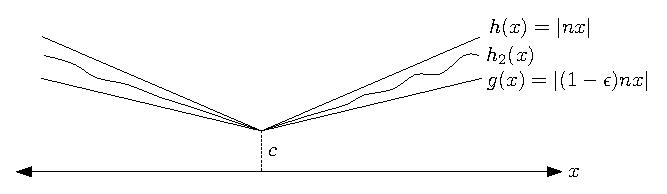
\includegraphics{trivial}\end{center}
\caption{The function $g$ is an approximation of $h$ and
of $h_2$.}\figlabel{trivial}
\end{figure}

Let $f$ be a non-negative convex function and let $f'$ be the first
derivative of $f$.  Assume that $f'(x)$ is defined for all but a
finite number of values of $x$ and that $|f'(x)|\le n$ for all $x$ in
the domain of $f'$.  For convenience, we define the \emph{right
derivative} $f^*(x)$ as follows: If $f'(x)$ is defined, then
$f^*(x)=f'(x)$.  Otherwise, $f^*(x)=\lim_{\delta\rightarrow 0+}
f'(x+\delta)$.  To avoid overly long qualifications we will abuse
standard terminology slightly and call $f^*(x)$ the \emph{slope} of
$f$ at $x$.

Let $a$ be the largest value at which the slope of $f$ is at most
$-(1-\eps)n$, i.e., 
\[
a=\max\{x:f^*(x)\le -(1-\eps)n \} \enspace .
\]
(Here, and throughout, we use the convention that
$\max\emptyset=-\infty$ and $\min\emptyset=\infty$.)  Similarly, let
$b=\min\{x:f^*(x)\ge (1-\eps) n\}$.  Then, from the above discussion,
it is clear that the function
\begin{equation}
 g(x) = \left\{\begin{array}{ll}
                 f(a) + (1-\eps)(a-x)n & \mbox{if $x\le a$} \\
                 f(b) + (1-\eps)(x-b)n & \mbox{if $x\ge b$} \\
                 f(x)   & \mbox{otherwise} \eqlabel{approx}
 \end{array}\right.
\end{equation}
is an $\eps$-approximation of $f$ (see \figref{approx}).

\begin{figure}
\begin{center}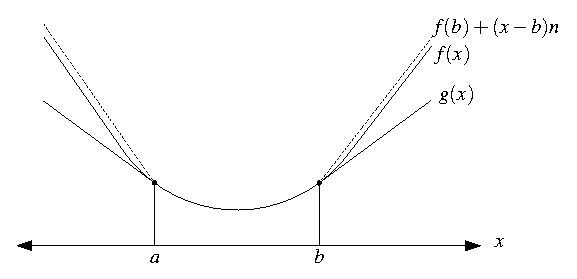
\includegraphics{approx}\end{center}
\caption{The function $g$ is a $(1-\eps)$ approximation of
$f$.}\figlabel{approx}
\end{figure}

\Eqref{approx} tells us that we can approximate $f$ by using two
linear pieces and then recursively approximating $f$ in the range
$(a,b)$.  However, in the range $(a,b)$, $f^*$ is in the range
$(-(1-\eps)n, (1-\eps)n)$.  Therefore, if we recurse $\lceil \log_E
n\rceil$ times, we obtain a function $g$ with $O(\log_E n) =
O((1/\eps) \log n)$ linear pieces that approximates $f$ at all points
except possibly where $f^*$ is less than 1.

\begin{thm}\thmlabel{approx}
Let $f$ and $f^*$ be defined as above.  Then there exists a piecewise-linear
function $g(x)$ with $O((1/\eps)\log n)$ pieces that is an
$\eps$-approximation to $f(x)$ at all values where $|f^*(x)|\ge 1$.
\end{thm}

For some special classes of convex functions (for example, the
\emph{extent} of a line arrangement \cite{ah01}) it is possible to
find $\eps$-approximations whose size is only a function $\eps$, and
is independent of $n$.  As we will see in \secref{lower-bound}, this is
not the case for the general class of convex functions we consider here.

\section{Data Structures}\seclabel{ds}

In this section, we consider the consequences of \thmref{approx} in
terms of data structures for approximating convex functions.  By
storing the pieces of $g$ in an array sorted by $x$ values, we obtain
the following.

\begin{thm}
Let $f$ and $f^*$ be defined as in \secref{approx}.  Then there exists
a data structure of size $O((1/\eps) \log n)$ that can compute an
$\eps$-approximation to $f(x)$ in $O(\log (1/\eps) + \log \log n)$
time for any query value $x$ where $|f^*(x)|\ge 1$.
\end{thm}

Next, we consider a more dynamic model, in which the function $f$ is
updated over time.  In particular, we consider the following
operations that are applied to the initial function $f(x)=0$, for all
$x\in\Real$.

\begin{enumerate}
\item $\textsc{Query}(x)$: Return an $\eps$-approximation to
  $f(x)$.

\item $\textsc{Insert}(a)$: Increase the slope of $f$ by 1 in the
  range $(a,\infty)$, i.e., set $f(x)\gets f(x)+x-a$ for all $x\in
  [a,\infty)$.

\item $\textsc{Delete}(x)$: Decrease the slope of $f$ by 1 in the
  range $(x,\infty)$.  In order to maintain convexity, the number of
  calls to $\textsc{Delete}(x)$ may not exceed the number of calls to
  $\textsc{Insert}(x)$ for any value of $x$.
\end{enumerate}

Note that a sequence of \textsc{Insert} and \textsc{Delete} operations
can only produce a monotonically increasing function $f$ whose slopes
are all integers.  This is done to simplify the exposition of the data
structure.  If an application requires that $f$ be allowed to decrease
and increase then two data structures can be used and their results
summed.  \comment{Also, if non-integer slopes are required then the data
structure and algorithms are easily modified to support an additional
parameter $\delta$, $0<\delta\le 1$ to the \textsc{Insert} and
\textsc{Delete} procedures that specifies the amount by which the
slope is to be increased or decreased, respectively.}

The function $f$ has some number $m\le n$ of breakpoints, where the slope
of $f$ changes.  We store these breakpoints in a balanced search tree
$T$, sorted by $x$-coordinate.  With each breakpoint $x$, we also
maintain the value $\Delta(x)$ by which the slope of $f$ increases at
$x$.  In addition, we link the nodes of $T$ in a doubly-linked list,
so that the immediate successor and predecessor of a node can be found
in constant time.  It is clear that $T$ can be maintained in $O(\log
n)$ time per operation using any balanced search tree data structure.

In addition to the search tree $T$, we also maintain an array $A$ of
size $O((1/\eps) \log n)$ that contains the piecewise linear
approximation of $f$.  The $i$th element in this array contains the
value $x_i$ such that $x_i=\min\{x:f^*(x) \ge E^i \}$, a pointer to
the node in $T$ that contains $x_i$, and the values of $f(x_i)$ and
$f^*(x_i)$, i.e., the value of $f$ at $x_i$ and slope of $f$ at $x_i$.
To update this array during an \textsc{Insert} or \textsc{Delete}
operation, we first update the values of $f(x_i)$ and $f^*(x_i)$ for
each $i$.  Since there are only $O((1/\eps) \log n)$ array entries,
this can be done in $O((1/\eps) \log n)$ time.

Next, we go through the array again and check which values of $x_i$
need to be changed (recall that $x_i=\min\{x:f^*(x) \ge E^i \}$).
Note that, since \textsc{Insert} or \textsc{Delete} can only change
the value of $f^*(x)$ by 1, if the value of $x_i$ changes then it
changes only to its successor or predecessor in $T$.  Since the nodes
of $T$ are linked in a doubly-linked list, and we store the values of
$f(x_i)$ and $f^*(x_i)$ we can detect this and update the value of
$x_i$, $f(x_i)$ and $f^*(x_i)$ in constant time.  Therefore, over all
array entries, this takes $O((1/\eps) \log n)$ time.

To evaluate an approximation to $f(x)$, we do a binary search on $A$
to find the index $i$ such that $[x_i,x_{i+1})$ contains $x$ and then
output $f(x_i) + (x-x_i)f^*(x_i)$.  By the choice of $x_i$, this is a
$\eps$-approximation to $f(x)$. 

Thus far, we have described a data structure whose size is
$O(n+(1/\eps)\log n)$.  However, if $(1/\eps)\log n > n$ then a
simpler data structure, namely the one that stores the function $f$
explicitly in an array achieves the same update  and search time
bounds and requires only $O(n)$ space.  This completes the proof of:

\begin{thm}
There exists a data structure of size $O(n)$ that supports the
operations \textsc{Insert}, \textsc{Delete} in $O((1/\eps) \log n)$
time and \textsc{Query} in $O(\log (1/\eps) + \log \log n)$ time,
where $n$ is the maximum slope of the function $f$ being maintained.
\end{thm}

\noindent\textbf{Remark:} In some cases, it may be desirable to
maintain functions that have arbitrarily small or large changes in
their slopes.  That is, the operations \textsc{Insert} and
\textsc{Delete} come with an extra parameter $\delta$ that specifies
by how much to increase or decrease the slope.  In this case, we can
still use a similar approach, but the update time bound becomes
$O((1/\eps)\log n\log m)$, where $m$ is the number of locations at
which the slope changes.  This running time comes from the fact that,
when a relatively large value of $\delta$ is used, the locations of
the $x_i$'s may change by a lot, and each of these $O((1/\eps)\log n)$
values requires a search in a tree of size $m$.



\section{A Lower Bound on Storage}\seclabel{lower-bound}

Recently, several approximation schemes have been presented in which
the size of the data structure is a function only of $\eps$ and not of
any of the other input parameters \cite{ah01,i01}.  In this
section, we show that such a result is not possible in our setting.
Indeed, the amount of space required is a function of the maximum
slope $n$, and the maximum value $X$ at which the slope is allowed to
increase.

For $i=1,\ldots,M$ let $x_i=((1-\eps)/\eps)^i$, let $D=1/(1-2\eps)$ and let
$m=\lfloor\log_D n\rfloor$.  Let $\{j_1,\ldots,j_m\}$ be a subset of
$\{1,\ldots,M\}$.  We will show that $j_1,\ldots,j_m$ can be encoded
as a piecewise linear non-decreasing convex function $f$ whose maximum
slope is bounded by $n$ and whose pieces begin and end only at the
elements of $\{x_1,\ldots,x_M\}$.  Furthermore, this encoding is
robust in the sense that, given only an $\eps$-approximation $g$
of $f$ we can use to $g$ to recover the subset of $\{1,\ldots,M\}$
used to define $f$.  Thus, we conclude that any data structure
must use $\log {M\choose m}\approx (1/\eps)\log n\log M$ bits of
storage. 

We define the convex function $f$ as follows:
\begin{enumerate}
\item For $x\in [-\infty,0)$, $f(x)=0$.
\item For $x\in (x_{j_i},x_{j_{i+1}})$, $f(x)$ has slope $D^j$.
\item For $x>j_m$, $f(x)$ has slope $n$.
\end{enumerate}

Next we show how, given only an approximation $g$ of $f$, we can
completely reconstruct the function $f$. Suppose we have already
reconstructed the values $f(x_1),f(x_2),\ldots,f(x_{i})$ and we 
now want to reconstruct the value $f(x_{i+1})$.  More precisely, we
have already determined the slope $D^j$ of $f(x)$ for $x\in
(x_{i-1},x_{i})$ and we need to decide whether the slope of $f(x)$ for
$x\in(x_i,x_{i+1})$ is $D^j$ or $D^{j+1}$.  If the new slope is $D^j$
then, because $f$ and $f^*$ are non-decreasing and $f(0)=0$, we have
\begin{eqnarray*}
   g(x_{i+1}) & \le & f(x_{i+1}) \\
    & < & x_{i+1}D^j \enspace . 
\end{eqnarray*}
On the other hand, if the new slope is $D^{j+1}$ then
\begin{eqnarray*}
   g(x_{i+1}) 
    & \ge & (1-\eps)f(x_{i+1}) \\
    & = & (1-\eps)(f(x_i) + (x_{i+1}-x_i)D^{j+1}) \\
    & \ge & (1-\eps)(x_{i+1}-x_i)D^{j+1} \\ 
    & = & \left(\frac{1-\eps}{1-2\eps}\right)(x_{i+1}-x_i)D^{j} \\ 
    & = &
\left(\frac{1-\eps}{1-2\eps}\right)\left(\left(\frac{1-\eps}{\eps}\right)x_i-x_i\right)D^{j} \\ 
    & = & \left(\frac{1-\eps}{\eps}\right)x_iD^j \\
    & = & x_{i+1}D^j \enspace .
\end{eqnarray*}
Thus, we can determine if the slope (and hence the value) of $f(x)$
for $x\in (x_i,x_{i+1})$ by testing if $g(x_{i+1}) < x_{i+1}D^j$.  We
conclude that we can reconstruct the entire function $f$, and
therefore the values $j_1,\ldots,j_m$, given only a function $g$ that
is an $\eps$-approximation to $f$. 

\begin{thm}
Let $m=\lfloor\log_E n\rfloor$.  Any data structure that can represent
an $\eps$-approximation to an increasing, piecewise-linear convex
function whose slopes are integers in the range $[0,n]$ and whose
slope changes only at integers in the range $[0,((1-\eps)/\eps)^M]$
requires $\log {M\choose m}$ bits of storage, in the worst case.
 \end{thm}

\begin{rem}
Some readers may complain that the function used in our lower bound
construction uses linear pieces whose lengths are exponential in $M$,
so representing a single such value requires $\Omega(M)$ bits.
However, all these values are powers of $(1-\eps)/\eps$ and can
therefore be encoded using $O(\log M)$ bits each using, e.g., a
floating point representation.
\end{rem}

\section{Applications}\seclabel{applications}

Next, we consider applications of our approximation technique for
convex functions to the problem of approximating sums of distances in
$d$ dimensions.  Let $S$ be a set of $n$ points in $d$ dimensions.
The \emph{Fermat-Weber weight} of a point $q\in\Real^d$ is
\[
   \fw(p) = \sum_{q\in S} \|pq\| \enspace ,
\]
where $\|pq\|$ denotes the distance between points $p$ and $q$. Of
course, different definitions of distance (e.g., Euclidean distance,
Manhattan distance) yield different Fermat-Weber weights.

\subsection{The 1-dimensional Case}

One setting in which distance is certainly well defined is in one
dimension.  In this case,
\[ 
\|pq\| = |p-q| \enspace ,
\]
so the Fermat-Weber weight of $x$ is given by
\[
   \fw(x) = f(x) = \sum_{y\in S} |x-y|  \enspace .
\]
Note that the function $f$ is convex (it is the sum of $n$ convex
functions) and has slopes bounded below by $-n$ and above by $n$, so
it can be approximated using the techniques \secref{ds}.  Furthermore,
adding or removing a point $p$ to/from $S$ decreases the slope of $f$
by 1 in the range $(-\infty,p)$ and increases the slope of $f$ by 1 in
the range $(p,\infty)$, so the dynamic data structure of the previous
section can be used to maintain an $\eps$-approximation of $f$ in
$O(\log_E n)= O((1/\eps) \log n)$ time per update.

Given the set $S$, constructing the $\eps$-approximation for $f$
can be done in $O(n/\eps)$ time by a fairly straightforward
algorithm:  Using a linear-time selection algorithm, one finds the
elements of $S$ with ranks $\lfloor\eps n/2\rfloor$ and
$\lceil(1-\eps/2) n\rceil$.  These are the values $a$ and $b$ in
\eqref{approx}.  Once this is done, the remaining problem has size
$(1-\eps) n$ and is solved recursively.  Although some care is
required to compute the values $f(a)$ and $f(b)$ at each stage, the
details are not difficult and are left to the interested reader.

\begin{rem} 
A general (and surprising) result of Agarwal and Har-Peled \cite{ah01}
implies that the Fermat-Weber weight of points in one dimension can
actually be $\eps$-approximated by a piecewise-linear function with
$O(1/\eps)$ pieces, independent of $n$.  However, it is not clear how 
easily this approach
can be made dynamic to handle insertion and deletions of points. 
The data structure of the previous section is also (arguably)
considerably simpler.
\end{rem}

\subsection{The Manhattan Case}

The Manhattan distance between two points $p$ and $q$ in $\Real^d$ is
\[
\|pq\|_1 = \sum_{i=1}^d |p_i-q_i| \enspace ,
\]
where $p_i$ denotes the $i$th coordinate of point $p$.  We simply
observe that Manhattan distance is the sum of $d$ 1-dimensional
distances, so the Fermat-Weber weight under the Manhattan distance can
be approximated using $d$ one-dimensional data structures.

\subsection{The Euclidean Case}

The Euclidean distance between two points $p$ and $q$ in $\Real^d$ is
\[
\|pq\|_2 = \left(\sum_{i=1}^d (p_i-q_i)^2\right)^{1/2} \enspace .
\]

A general technique used to approximate Euclidean distance is to use a
polyhedral distance function, in which the unit sphere is replaced
with a polyhedron that closely resembles a sphere.  For example, the
Manhattan distance function is a polyhedral distance function in which
the unit sphere is replaced with a unit hypercube.  Although this
technique works well when $d$ is small, such metrics generally require
a polyhedron with a number of vertices that is exponential in $d$,
making them less well-suited for high dimensional applications.

Another technique, that works well when $d$ is very large (greater
than $\log n$), and for many distance functions, is that of random
projections \cite{i01}. Here, a random $O(\log n)$-flat is chosen and
the points of $S$ are projected orthogonally onto this flat.  With
high probability, all interpoint distances are faithfully preserved
after the projection, so the problem is reduced to one in which the
dimension of the point set is $O(\log n)$ (see
Ref.~\cite[Lemma~3]{i01} for details).  A related technique is to
project the points onto a set of randomly chosen lines and use the sum
of distances in these projections as an estimate of the interpoint
distance \cite{k97}.  The drawback of these techniques for
Fermat-Weber type problems is that they only guarantee that each
individual point in $\mathbb{R}^d$ has its Fermat-Weber weight
$\eps$-approximated with high probability.  This makes them less
well-suited for use in search algorithms whose correctness relies on
access to an $\eps$-approximation for the Fermat-Weber weight of every
point (or many points) in $\mathbb{R}^d$.

In this section we show that both of the above strategies can be used
in conjunction with our approximation scheme for convex functions.


\subsubsection{A Randomized Approximation}

Here we describe a technique based on Kleinberg's method of projecting
onto random lines \cite{k97}.  Consider the following experiment: Pick
a random point $v$ on the surface of the unit sphere
$\mathbb{S}^{d-1}$ in $\mathbb{R}^d$ and consider the line $\ell$
through the origin and $v$. For two points $p,q\in\mathbb{R}^d$,
project $p$ and $q$ orthogonally onto $\ell$ to obtain points $p_\ell$
and $q_\ell$, respectively. Consider the random variable
$|p_\ell-q_\ell|$ that measures the distance between the two projected
points.  Then $\E[|p_\ell-q_\ell|]=c_d\|pq\|_2$, where
$c_d=\Theta(1/\sqrt{d})$ is a constant whose value is discussed in
\appref{luc}.  

Let $f(p)$ denote the Fermat-Weber weight of $p$ under the Euclidean
distance function.  Choose $k$ random lines $\ell_1,\ldots,\ell_k$ as
described above and let $f_i(p)$ denote the Fermat-Weber weight of the
1-dimensional point $p_{\ell_i}$ in the 1-dimensional set
$S_{\ell_i}$.  That is,
\[
     f_i(p) = \sum_{q\in S} |p_{\ell_i}-q_{\ell_i}| \enspace .
\]
Then $f_i(p)$ is a random variable that may take on any value in the
range $[0,c_df(p)]$.  In particular, $f_i(p)$ has an expected value 
\[
   \E[f_i(p)]=c_df(p) \enspace . 
\] 

Next consider the normalized average function 
\[ g(p) = \frac{1}{kc_d}\times\sum_{i=1}^k f_i(p) \] 
that approximates the
Fermat-Weber weight under Euclidean distance.

\begin{lem}
$\Pr\{|g(p)-f(p)| \ge \delta f(p)\} = \exp(-\Omega(\delta^2k))$
\end{lem}

\begin{proof}
The value of $g(p)$ is a random variable whose expected value is
$f(p)$ and it is the sum of $k$ independent random variables, all of
which are in the range $[0,f(p)/c_d]$.  Applying Hoeffding's
inequality\footnote{Hoeffding's Inequality \cite{h63}: Let
$S_n=\sum_{i=1}^n X_i$ where $X_1,\ldots,X_n$ are
bounded independent bounded random variables such that $X_i\in[a_i,b_i]$ with probability 1.  Then, for any $t>0$,
$
    \Pr\{S_n - \E[S_n] \ge t\} 
   \le e^{-2t^2/\sum_{i=1}^n(b_i-a_i)^2}
$
and
$
    \Pr\{S_n - \E[S_n] \le -t\} 
   \le e^{-2t^2/\sum_{i=1}^n(b_i-a_i)^2} \enspace .
$
} and simplifying yields the desired
result.
\end{proof}

In summary, $g(p)$ is a $\delta$-approximation of $f(p)$ with
probability $1-e^{-\Omega(\delta^2k)}$.  Furthermore, $g(p)$ is the
sum of $k$ 1-dimensional Fermat-Weber weights which can be
$\eps$-approximated using the results of \secref{ds}.  This gives a
data structure of size $O(k(1/\eps)\log n)$ that can be constructed in
time $O(kn)$.  Queries in the data structure take
$O(k(\log(1/\eps)+\log\log n))$ time and return an
$(\eps+\delta)$-approximation to the Fermat-Weber
weight of any point $p\in\mathbb{R}^d$ with probability at least
$1-e^{-\Omega(\delta^2k)}$. 

\subsubsection{A Deterministic Approximation}
\seclabel{ds-deterministic}

Next we show how to derandomize the data structure of the previous
section to obtain a data structure that guarantees an
$\eps$-approximation to $f(p)$ for \emph{every} point
$p\in\mathbb{R}^d$.  We do this by replacing the random points used in
the previous construction with $k$ points evenly distributed on
$\mathbb{S}^{d-1}$.  In particular, in \appref{pat} we show how to
find $k=O((d^3/\delta^4)\log (d/\delta))$ points on $\mathbb{S}^{d-1}$
to obtain a set of lines $\ell_1,\ldots,\ell_k$ such that
\[
      (1-\delta)|pq|\le \frac{1}{kc_d} \sum_{i=1}^k |p_{\ell_i}-q_{\ell_i}| 
      \le (1+\delta)|pq| 
\]
for every $p,q\in\mathbb{R}^d$.

Thus, we can maintain a $\delta$-approximation to the Fermat-Weber
function $f$ by maintaining $k$ 1-dimensional data structures.  To
summarize, this gives us a data structure of size
$O(((d^3/\delta^{4})\log(d/\delta))(1/\eps)\log n)$ that can be constructed in
$O(((d^3/\delta^4)\log(d/\delta)n)$ time and that can return an
$(\eps+\delta)$-approximation to $f(p)$ for any $p\in\mathbb{R}^d$ in
$O(((d^3/\delta^{4})\log (d/\delta))(\log(1/\eps) + \log\log n))$ time.

\subsection{Clustering and Facility Location}

Bose \etal\ \cite{bmm02} describe data structures for approximating
sums of distances.  They show how, for fixed $d$ and $\eps$, to
build a data structure in $O(n\log n)$ time that can
$(1-\eps)$-approximate the Fermat-Weber weight of any point in $O(\log
n)$ time.  These results have a leading constant of the form
$\Omega((1/\eps)^d)$.

The same authors give applications of their data structures to a
number of facility-location and clustering problems, including
evaluation of the Medoid and AverageDistance clustering measures, the
Fermat-Weber problem, the constrained Fermat-Weber problem, and the
constrained obnoxious facility-location problem.  All of these
applications also work with the data structure of \secref{ds}, many
with improved running times.  

A summary of these results is given in \tabref{applications}, which
shows running times assuming $\eps$ and $d$ are fixed constants,
independent of $n$.  The results in the right-hand column are obtained
simply by using the methods described by Bose \etal\ in combination
with the deterministic data structure of \secref{ds-deterministic}.
It is worth noting that the leading constant in the algorithms
obtained this way is only 
$O((d^3/\eps^4)\log (d/\eps))$, while the leading constant in the
algorithm by Bose \etal\ is $\Omega((1/\eps)^d)$.

\begin{table}
\begin{minipage}{\textwidth}
\begin{center}\begin{tabular}{l|cccc}
Problem      & Previous $\eps$-approx. & Ref. & New $\eps$-approx. \\ \hline
Average distance  & $^a$ $O(n)$ $O(n\log n)$ & 
    \cite{bmm02,i99} & $O(n\log\log n)$ \\
Medoid (1-Median)  & $^a$ $O(n)$ $O(n\log n)$ & 
    \cite{bmm02,i99} & $O(n\log\log n)$ \\
Discrete Fermat-Weber  & $^a$ $O(n)$ $O(n\log n)$ & 
    \cite{bmm02,i99} & $O(n\log\log n)$ \\
Fermat-Weber  & $^b$ $O(n)$ $O(n\log n)$ & 
    \cite{bmm02,i99} & $O(n)$ \\
Constrained Fermat-Weber  & $^b$ $O(n)$ $O(n\log n)$ & 
    \cite{bmm02,i99} & $O(n)$ \\
Constrained OFL  & $^a$ $O(n)$ $O(n\log n)$ & 
    \cite{bmm02,i99,k97} & $O(n\log\log n)$ 
\end{tabular}\end{center}
\footnotetext[1]{The first running time refers to a randomized algorithm that
  outputs a  $(1-\eps)$-approximation with constant probability.}
\footnotetext[2]{The first running time refers to a randomized algorithm that outputs a
  $(1-\eps)$-approximation with high probability, i.e., with probability
  $1-n^{-c}$, for some $c>0$.}
\end{minipage}
\caption{Applications of the data structure for evaluating the Fermat-Weber
  weights of points under the Euclidean distance function.}
\tablabel{applications}
\end{table}


\comment{
\section{Summary and Conclusions}\seclabel{conclusions}

We have given static and dynamic data structures for approximating
convex functions of one variable whose slopes are bounded.  These data
structures have applications to problems involving sums of distances
in $d$ dimensions under both the Manhattan and Euclidean distance
functions.  In developing these applications we have arrived at a
technique of independent interest, namely that of approximating
Euclidean distance as the sum of several Manhattan distances under
several different orientations of the coordinate system.
}

\bibliographystyle{plain}
\bibliography{curves}


\appendix
\section{The value of $\mathbf{c_d}$}
\applabel{luc}

The value of $c_d$ that appears in \secref{applications} is given by
\[
  c_d = \E \left[|x_1| \right] \enspace ,
\]
where $(x_1,\ldots,x_d)$ is a point taken from the uniform
distribution on the unit sphere $\mathbb{S}^{d-1}$ in $\mathbb{R}^d$.
We observe that $(x_1^2,\ldots,x_d^2)$ is distributed as 
\[
\left(\frac{N_1^2}{N^2},\ldots,\frac{N_d^2}{N^2}\right) \enspace ,
\]
where $N^2=\sum_{i=1}^d N_i^2$ and $(N_1,\ldots,N_d)$ are i.i.d.\
$\mathrm{normal}(0,1)$.  Clearly,
\[
\frac{N_1^2}{N^2} = \frac{N_1^2}{N_1^2+\sum_{i=2}^dN_i^2}
  \stackrel{\mathcal{L}}{=} \frac{G(\frac{1}{2})}{G(\frac{1}{2})+G(\frac{d-1}{2})}
\]
where $G(\frac{1}{2})$, and $G(\frac{d-1}{2})$ are independent
$\mathrm{gamma}(\frac{1}{2})$ and $\mathrm{gamma}(\frac{d-1}{2})$
random variables, respectively.  Thus, $N_1^2/N$ is distributed as a
$\mathrm{beta}(\frac{1}{2},\frac{d-1}{2})$ random variable,
$\beta(\frac{1}{2},\frac{d-1}{2})$.  We have:
\begin{eqnarray*}
\E\left[|x_1|\right]
 & = & \E\left[\sqrt{\beta\left(\frac{1}{2},\frac{d-1}{2}\right)}\right] \\
 & = & \int_0^1\frac{x^{\frac{1}{2}-1}(1-x)^{\frac{d-1}{2}-1}}
                    {B(\frac{1}{2},\frac{d-1}{2})}\cdot\sqrt{x} \quad dx\\
 & = & \frac{B(1,\frac{d-1}{2})}{B(\frac{1}{2},\frac{d-1}{2})}\\
\comment{ & = & d\cdot 
       \frac{\Gamma(\frac{d-1}{2})}
            {\Gamma(\frac{d+1}{2})} \cdot
       \frac{\Gamma(\frac{d}{2})}
            {\Gamma(\frac{1}{2})\cdot\Gamma(\frac{d-1}{2})} \\
 & = & \frac{d\Gamma(\frac{d}{2})}
            {\Gamma(\frac{1}{2})\cdot\Gamma(\frac{d+1}{2})} \\ 
 & = & \frac{2\Gamma(\frac{d}{2}+1)}
            {\Gamma(\frac{1}{2})\cdot\Gamma(\frac{d+1}{2})} \\
}
 & = & \frac{2}{dB(\frac{1}{2},\frac{d+1}{2})} \enspace , 
\end{eqnarray*}
where $B(a,b)$ is the beta function.

From Mitrinovic \cite[p.~286]{m70}, we note:
\begin{eqnarray}
\frac{2}{dB(\frac{1}{2},\frac{d+1}{2})} & \ge &
  \frac{1}{d}\sqrt{\frac{d}{2}+\frac{1}{4}+\frac{1}{16d+32}}\cdot 
     \frac{1}{\Gamma(\frac{1}{2})} \\
 & = & \frac{2}{d}\sqrt{\frac{d}{2}+\frac{1}{4}+\frac{1}{16d+32}}\cdot
      \frac{1}{\sqrt{\pi}} \\
 & \ge & \frac{1}{d}\sqrt{\frac{2d+1}{\pi}} \enspace .
\end{eqnarray}

Furthermore,
\begin{eqnarray*}
\E\left[|x_1|\right] 
  & \le & \frac{1}{d}\frac{d+1}{\sqrt{\pi}\cdot\sqrt{\frac{d}{2}+
                       \frac{3}{4}+\frac{1}{16d+48}}} \\
  & \le & \frac{1}{d}\frac{2(d+1)}{\sqrt{\pi}\cdot\sqrt{2d+3}} \\ 
  & \le & \frac{1}{d}\sqrt\frac{2(d+1)}{\pi} \enspace . 
\end{eqnarray*}

In summary,
\[
\frac{1}{d}\sqrt\frac{2d+1}{\pi} \le c_d = \frac{1}{d}\frac{2\Gamma(\frac{d}{2}+1)}
                            {\sqrt{\pi}\cdot\Gamma(\frac{d+1}{2})}
 \le \frac{1}{d}\sqrt{\frac{2(d+1)}{\pi}} \enspace .
\]

\section{Choosing the Lines and Weights}
\applabel{pat}
\newcommand{\ccap}{\mathrm{cap}}
\newcommand{\Sd}{\mathbb{S}^{d-1}}
\newcommand{\area}{\mathrm{vol}}

From the previous appendix, we know that $c_d$ is the expected
absolute value of the $x$-coordinate of a point $v$ chosen uniformly
at random from $\Sd$.  Let $\ccap(\theta)$ denote the spherical cap of
angular radius $\theta$ obtained by intersecting $\Sd$ with the
halfspace $x_1\ge\cos(\theta)$ and let $\area(C)$ denote the surface
area (volume) of the spherical cap $C$.  Then, we have the following
inequalities for $c_d$,
\begin{eqnarray*}
   c_d & = & \E[|x_1|] \\ 
   & = & 2\sum_{i=1}^m \Pr\left\{x\in 
             \ccap\left(\frac{i\pi}{m}\right) \setminus
                  \ccap\left(\frac{(i-1)\pi}{m}\right)\right\}\cdot
              \E\left[x_1\mid x\in
              \ccap\left(\frac{i\pi}{m}\right) \setminus
                  \ccap\left(\frac{(i-1)\pi}{m}\right)
              \right] \\
   & \le & \frac{2}{\area(\Sd)}\cdot
                  \sum_{i=1}^m \cos\left(\frac{(i-1)\pi}{2m}\right)
                  \left(\area\left(\ccap\left(\frac{i\pi}{2m}\right)\right)-
                     \area\left(\ccap\left(\frac{(i-1)\pi}{2m}\right)\right)
                  \right) \\
   & \le & \frac{2}{\area(\Sd)}\cdot
                  \sum_{i=1}^m \left(\cos\left(\frac{i\pi}{2m}\right)+\frac{2}{m}\right)
                  \left(\area\left(\ccap\left(\frac{i\pi}{2m}\right)\right)-
                     \area\left(\ccap\left(\frac{(i-1)\pi}{2m}\right)\right)
                  \right) \\
   & = & \frac{2}{\area(\Sd)}\cdot
                  \sum_{i=1}^m \cos\left(\frac{i\pi}{2m}\right)
                  \left(\area\left(\ccap\left(\frac{i\pi}{2m}\right)\right)-
                     \area\left(\ccap\left(\frac{(i-1)\pi}{2m}\right)\right)
                  \right) + \frac{2}{m} \\
   & \le & c_d + \frac{2}{m}  \enspace .
\end{eqnarray*}

Using the theory of $\eps$-approximations \cite[Chapter~4]{c00}, it is
possible, for any $r\ge 1$ to find a set $S$ of $k=O(dr^2\log dr)$
points on $\Sd$ such that, for \emph{any} spherical cap $C$
\[
    \left|\frac{\area(C)}{\area(\Sd)} - \frac{|C\cap S|}{|S|} \right| 
              \le \frac{1}{r}  \enspace 
\]
and by increasing the size of $S$ by a constant factor we may assume
that $S$ is symmetric ($x\in S$ iff $-x\in S$).
Let $S$ be such a set of points and consider the average
$x$-coordinate of an element in $S$.\footnote{The $x$-coordinate $x_1$
in this argument is simply a placeholder for the projection of $p-q$
onto $x$. That is, we are assuming without loss of generality that
$p-q=(1,0,0,\ldots,0)$, so that $p\cdot x - q\cdot x=(p-q)\cdot x=x_1$.}
\begin{eqnarray*}
\frac{1}{|S|}\cdot \sum_{x\in S} |x_1|
  \comment{ & = & \frac{2}{|S|}\cdot\sum_{i=1}^m
          \sum\left\{x_1: x\in
              S\cap\ccap\left(\frac{i\pi}{m}\right) 
                \setminus\ccap\left(\frac{(i-1)\pi}{m}\right)
          \right\} \\ }
  & \le & \frac{2}{|S|}\cdot
         \sum_{i=1}^m\cos\left(\frac{(i-1)\pi}{m}\right)
           \left(
             \left|\ccap\left(\frac{i\pi}{m}\right)\cap S\right| -
             \left|\ccap\left(\frac{(i-1)\pi}{m}\right)\cap S\right|
           \right) \\
  & \le & \frac{2}{\area(\Sd)}\cdot
         \sum_{i=1}^m\cos\left(\frac{(i-1)\pi}{m}\right)
           \left(
             \area\left(\ccap\left(\frac{i\pi}{m}\right)\right) -
             \area\left(\ccap\left(\frac{(i-1)\pi}{m}\right)\right) +
             \frac{2\area(\Sd)}{r}
           \right) \\
  & \le & \frac{2}{\area(\Sd)}\cdot
         \sum_{i=1}^m\cos\left(\frac{(i-1)\pi}{m}\right)
           \left(
             \area\left(\ccap\left(\frac{i\pi}{m}\right)\right) -
             \area\left(\ccap\left(\frac{(i-1)\pi}{m}\right)\right)
           \right) + \frac{4m}{r} \\
  & \le & c_d + \frac{2}{m} + \frac{4m}{r} \\
  & = & c_d + \frac{3}{m} 
\end{eqnarray*}
where the last inequality follows by taking $r=4m^2$, in which case
$|S|=O(dm^4\log dm)$.  Taking $m=3/\delta c_d$ and using a symmetric
argument to the one above to obtain a lower bound, we obtain
\[
  1-\delta \le \frac{1}{c_d|S|}\cdot\sum_{x\in S}|x_1| \le 1 + \delta
\]
with $|S|=O((d^3/\delta^4)\log(d/\delta))$.  





\end{document}
